\begin{figure*}[t]
\centering
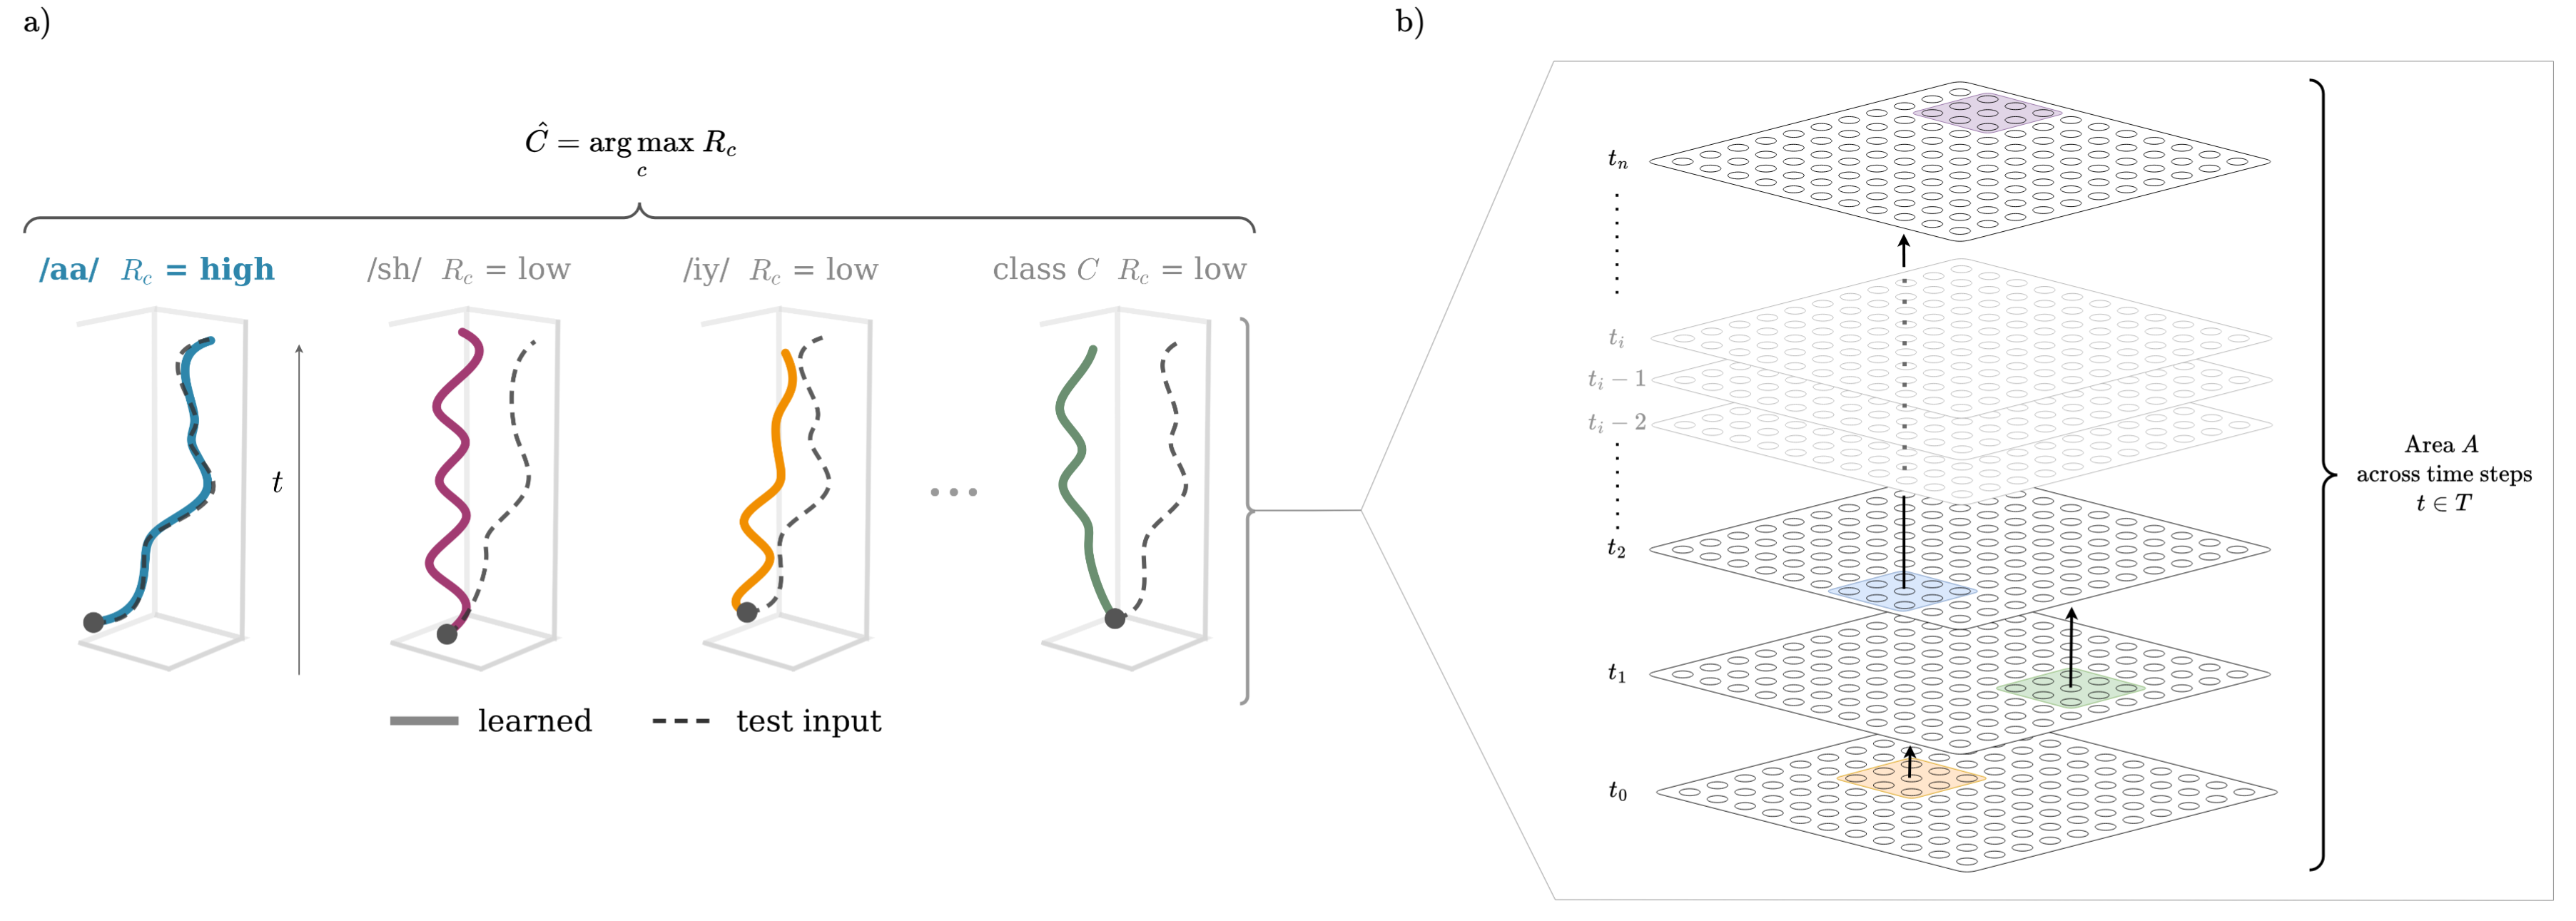
\includegraphics[width=0.9\textwidth]{figures/trajectories_with_detail_horizontal.png}
\caption{Trajectory-based resonance scoring. Each of $C$ per-class RecurrentAreas (a) has learned a characteristic trajectory through assembly space (solid, coloured). The same test input (dashed) is presented to all areas in parallel. The inset (b) shows the frame-by-frame operation: feedforward drive from the current input combines with recurrent drive from the previous assembly, and the top-$k$ neurons fire. The predicted class is the label of the area with the learned trajectory that most closely matches the input, as measured by the resonance score $R_c$.}
\vspace{-15pt}
\label{fig:trajectory}
\end{figure*}
